\documentclass[twocolumn, amsmath]{revtex4}


\usepackage{graphicx}


\begin{document}


\title{PHYS 605 Lab\#3} 

\author{Evin O'Shea}  % fill in your name here
\author{Morgan Daly}
\email{eco2000@unh.edu}  % add your email address 
\date{\today}  


\begin{abstract}

	

\end{abstract}

\maketitle

%
%  Now that the initial formatting and first-page details are set, let's add some relevant sections to the paper
%
\section{Background}
The first part of the lab was to learn to use the oscilloscope and to get two plots of AC voltage on the oscilloscope. Then the group was to modify the circuit and take note on how the changes affected the circuit. The group also was to take approximate quantitative data from the oscilloscope. The goal was to investigate the AC circuit and learn to use the tools associated with the second part of the lab.

The second part of the lab was to investigate the AC circuit quantitatively. The lab was to record measurements of how the AC circuit was affected by changes in the frequency of the circuit. As frequency was altered, the voltage across the capacitor was to be compared to the voltage accross the battery and the phase shift of the resistor and capacitor were to be recorded.


\section{Methodology}
The first part of the lab was simply to investigate AC circuits using an oscilloscope. The circuit was an RC circuit with a resistor and capacitor in series. One channel of the oscilloscope was connected in parallel with the whole circuit to see the output of the voltage source and the frequency of the source. The other channel was connected in parallel with the capacitor to see the voltage across the capacitor and the the phase shift of the voltage across the capacitor. Then, the group interchanged different resistors and capacitors as well as adjusted the frequency of the input voltage to record how the modifications affected the AC circuit.

The second part of the lab was to quantitatively investigate the behavior of the RC circuit as a function of frequency. The group used the same set up from the first part of the lab to measure the peak to peak voltage and the phase shift of the resistor and capacitor in the circuit as frequency was modified. The measurements were all recorded to be plot. The plot is a log plot, so the logarithm of the frequency is plotted against the gain in dB. The equation for gain in dB for voltage is shown below:

\begin{equation}
Gain (dB) = 20 log(\frac{V_{out}}{V_{in}}) = 20log(\frac{Z_2}{Z_1 + Z_2})
\end{equation}
This equation can be used to calculate the gain given the voltage from the input source and the voltage across the capacitor or it can be used to calculate expected values given the measurements of the imppedances.

\section{Results and Analysis}
The lab used a simple RC circuit. The circuit shown below does not include values for the resistance and capacitance of the elements because they were varied throughout the first part of the lab. The circuit is shown below:

\begin{figure}[h]  

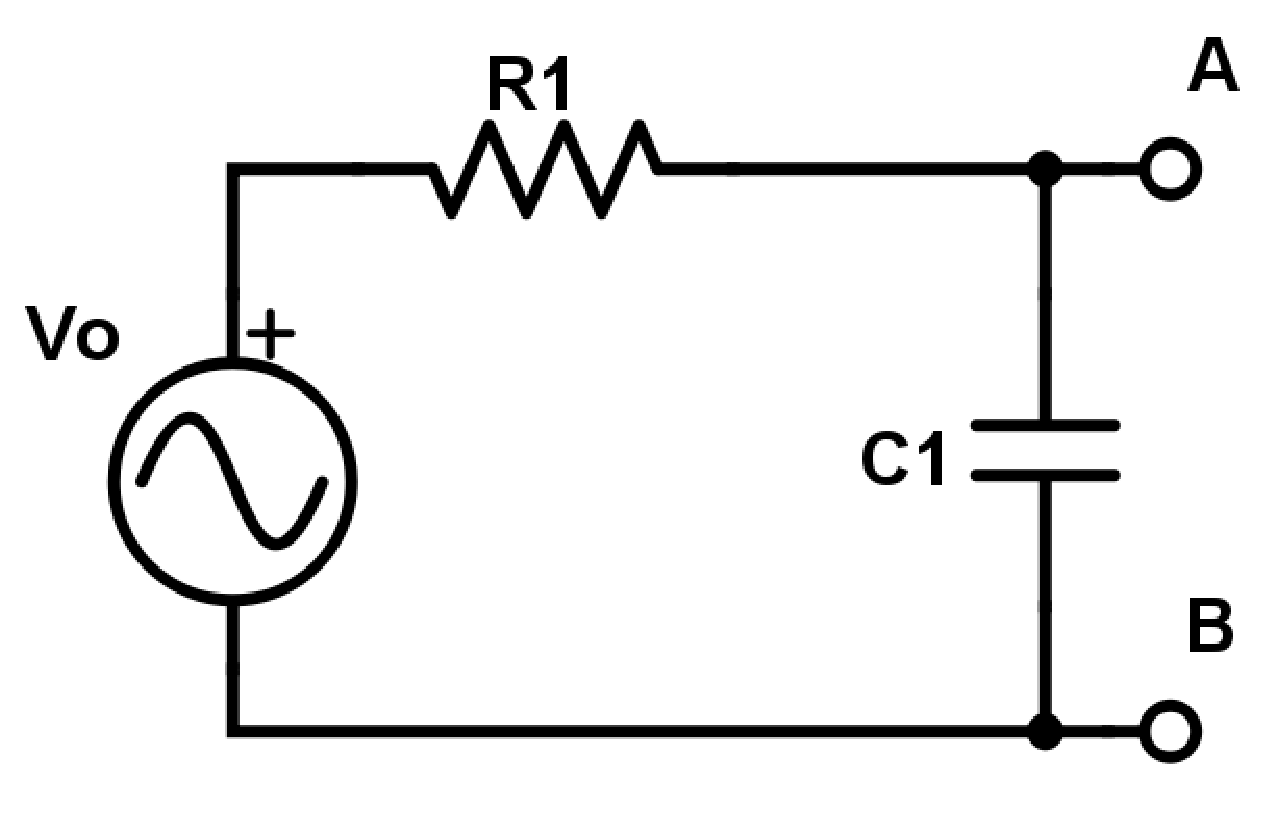
\includegraphics[scale = 0.4]{schemeit-project.eps}  
\end{figure}

The first objective of the lab was to display two voltage plots, one from the voltage source and one for the capacitor. The circuit made for this part included 10V (peak to peak) AC supplied to a 10k$\Omega$ resistor and a 4.7$\mu$F capacitor at 100Hz. This  yielded 300mV (peak to peak) potential accross the capacitor as well as about a 90 degree phase shift. The voltage plot is shown below:

\begin{figure}[h]  

\includegraphics[scale = 0.2]{pic.eps}  
\end{figure}

Next, the group made adjustments to the circuit and took notes on the changes in the plots. As the frequency was increased, the phase shift went up and then stayed at around 90 degrees. 

Then, the group changed the capacitor to a 0.518nF capacitor. The phase shift reduced to below 5 degrees and stayed that low as the frequency was varried. The peak to peak voltage accross the capacitor changed to 2.58 V (peak to peak). This means that as we decreased the capacitance, causing the voltage to increase and the phase shift to decrease.

Lastly, the group changed the resistor and increased it to a 98.4k$\Omega$. This increase in resistance yielded an increase in the voltage across the capacitor. This change did not affect the phase shift of the voltage across the capacitor much at all.

For the second part of the lab, the group re-visited the initial circuit. This circuit is shown above and included a 10.0k$\Omega$ resistor and a 4.7$\mu$F capacitor. The voltage source was set to 12.2V (peak to peak). The group started at about 10Hz and increased the frequency to over 10KHz. Each time the frequency was changed it was recorded along with the peak to peak voltages of the resistor and capacitor and their phase shifts. The data recorded is shown below:

\begin{center}
    \begin{tabular}{| l | l | l | l |}
    \hline
    frequency & $V_C (mV)$  & Gain (dB) & $\phi _C$ (degrees)  \\ \hline
 
    10.92Hz	& 3680	& -10.4	 & 78   \\ \hline
    24.04Hz 	& 1760	& -16.8	  & 90  \\ \hline
    71.73Hz   	& 720 	& -24.6	 & 97    \\ \hline
    97.66Hz   	& 440 	& -28.9	 & 95  \\ \hline
    337.8Hz    	& 134	& -39.2	 & 90 \\ \hline
    757.4Hz    	& 70.0	& -44.8	 & 92 \\ \hline
    1.066kHz   & 43.8	& -48.9	 & 80  \\ \hline
    5.102kHz  & 20.0	& -55.7	 & 87  \\ \hline
    12.99kHz   	& 16.0 & -57.6	 & 52   \\
    \hline
    \end{tabular}
\end{center}
The voltage across the resistor was always measured to be 12.2V and the phase shift was always less than 5 degrees. This is because there should be no phase shift across the resistor and because the resistance was high enough that most of the voltage was across the resistor. 

The gain values given from the measurements can also be compared to the expected gain  of the circuit. The gain is calculated using equation (1) where  $\frac{V_{out}}{V_{in}}$ is given from the imedances of the circuit elements. Measured versus expected values are shown below:
\begin{center}
    \begin{tabular}{| l | l | l | l |}
    \hline
    frequency &  $Gain_{meas}$  & $Gain_{exp}$ & \% Error  \\ \hline
 
    10.92Hz	& -10.4	& -12.5  &  16.8   \\ \hline
    24.04Hz 	& -16.8	& -18.17 &  7.53 \\ \hline
    71.73Hz   	& -24.6	& -26.9	&  6.92	    \\ \hline
    97.66Hz   	& -28.9	& -29.5	&  2.03	  \\ \hline
    337.8Hz    	& -39.2	& -40.1	&  2.24  \\ \hline
    757.4Hz    	& -44.8	& -47.0	&  4.68    \\ \hline
    1.066kHz   & -48.9	& -50.0	&  2.20	   \\ \hline
    5.102kHz   & -55.7	& -63.6	&  12.4	   \\ \hline
    12.99kHz   & -57.6	& -72.7	&  20.8	  \\
    \hline
    \end{tabular}
\end{center}

The data above shows that there was variance of the acccuracy of the oscilloscope and the measurements made. The sections with large error were the highest and lowest frequencies. It seemed that the oscilloscope could not make as accurate measurements when the voltage across the capacitor was very small; however, this does demonstrate that the gain values calculated are similar to the expected values for many data points. This means that the set up of the circuit was a success and the intended results were observed.

From the data shown above, a log plot (or Bode plot) can be made using calculated values of the gain (for output across the capacitor) and the log of the frequency. The gain was calculated using equation (1). The Bode plot of the gain is shown below:

\begin{figure}[h]  

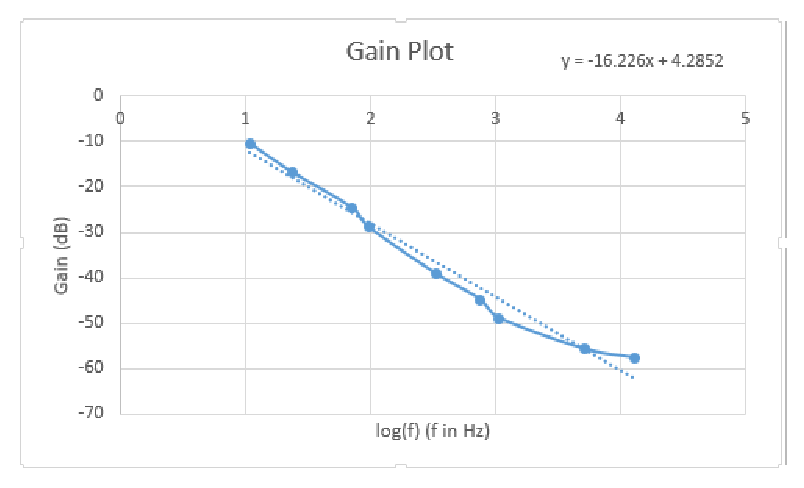
\includegraphics[scale = 0.5]{gainplot.eps}  
\end{figure}

As shown on the plot, the slope of the best fit line was -16.226. Since this line is only of negative gain values, the plot is of the "roll off" of the transfer function for the circuit. This means the "roll off" per decade is $16.226 \frac{dB}{decade}$. This indicates how the circuit works as a filter. High frequencies will have a negative gain, meaning they will be filtered out. The "roll off" characterizes how well the circuit cuts of frequencies. The frequencies used in the lab all had gains of less than -10. This means that the frequencies used were in the filtered range. This made it easy to determine the "roll off" and explains why the gain plot looks linear. It is simply a plot of the "roll off".

The phase shift of the output can also be plot versus the logarithm of the frequency. This was done below:

\begin{figure}[h]  

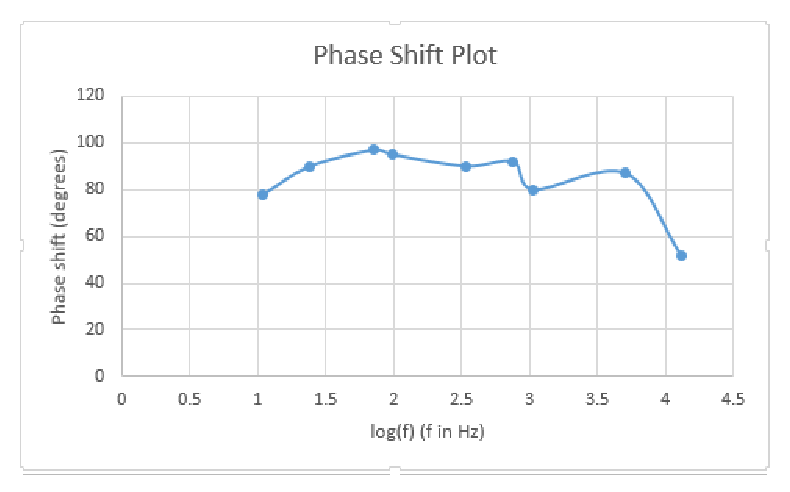
\includegraphics[scale = 0.5]{phaseshift.eps}  

\end{figure}

The phase shift did not seem to have a clear trend; however, this is because the range of frequencies measured were in the range around which the phase shift is stable. When a filter is past its -3dB point, the phase shift starts to level out at 90 degrees. The gain values and gain plot shows that the frequency range that was measured was part of the filtered range. This means that the phase shift will be roughly constant. This is why the phase shift did not change much over the frequencies measured. Furthermore, the phase shift values match the gain values in terms of expected outcome. Since the gain values are small, the phase shift should be near 90 degrees. There must have been some error in the oscilloscope as the phase shift should not have exceeded 90 degrees, but the phase shift was in the range that it was expected to be in.


\section{Conclusion}
The goal of the first part of the lab was to learn to use the oscilloscope and to invertigate the behavior of the AC circuit qualitatively and semi-quantitatively. The group successfully learned to use the oscilloscope and learned to plot multiple voltages on the display. Then, the group modified the circuit and learned that, in an RC circuit, if the resistance is increased or the capacitance is decreased, the voltage across the capacitor will increase. The group also learned, that decreasing capacitance will decrease the phase shift. The group observed proper AC circuit behavior. The lab group full completed this part of the lab correctly.

For the second part of the lab, the group was to analyze how an AC circuit behaved under changes in the input frequency of the voltage. The lab group successfully found the behavior of the circuit and characterized the "roll off" of the transfer function for the circuit. The group also found that the phase shift did not change much as the frequency was increased. The lab group discovered that the frequencies used in the lab were part of the filtered frequencies. This is why the phase shift did not change much and the gain plot looked linear. The lab group successfully completed the analyzation of the gain and phase shift of the circuit, as well as the "roll off" of the transfer function.


\end{document}
